For the purposes of this work, we implemented several conversational, directed gaze behaviors on a virtual agent. These behaviors include: (1) body orientation shifts to reconfigure the F-formation, (2) gaze behaviors to establish footing, and (3) gaze patterns to indicate listening, addressing, and floor release.

\subsection{Reconfiguring the F-formation}

The current work considers multiparty interaction centered on a virtual agent, which could be serving in the role of an instructor, storyteller, customer service representative, or non-player character in a multiplayer game. When a user approaches the agent, the latter must turn to face the user and thus invite them to engage in an interaction, creating a so-called vis-a-vis arrangement~\cite{kendon1990conducting}. If one or more avatar-embodied users are already present in the interaction, the agent must reorient its body such that it distributes its attention among the users as evenly as possible, creating an approximately circular arrangement.

\begin{figure}
\centering
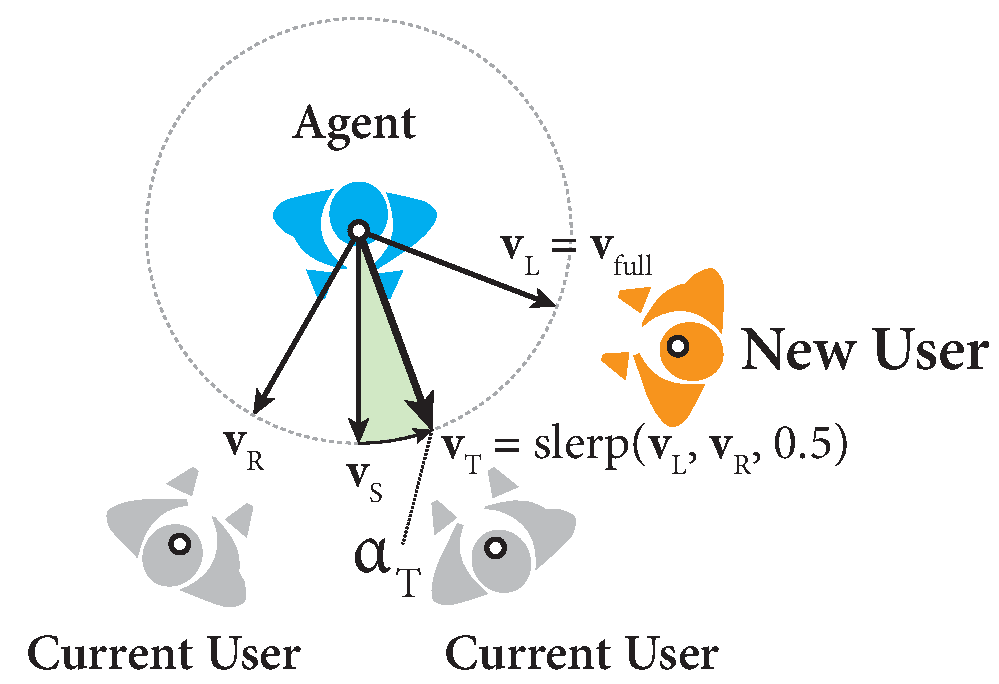
\includegraphics[width=0.75\textwidth]{conversationalrolegaze/Figures/FTorsoAlign.pdf}
\caption{Computing the torso alignment parameter $\alpha_T$ needed for the agent to reconfigure the F-formation when a new user has joined the interaction.}
\label{fig:FTorsoAlign}
\end{figure}

To implement these behaviors, we use our gaze shift model (Chapter~\ref{cha:GazeShiftModel}) to execute the body orientation shifts. When the first user approaches the agent, the agent performs a gaze shift toward the user with the head, torso, and whole-body alignment parameters all set to 1 ($\alpha_H = \alpha_T = \alpha_B = 1$). This results in the agent facing the user head-on. If users are already present in the interaction, the agent must perform a gaze shift toward the new user that evenly distributes its body orientation among all the users. We set $\alpha_H = 1$ and $\alpha_B = 1$ as before, whereas $\alpha_T$ must be set such that the agent ends up oriented toward the midpoint between the leftmost and rightmost user. The procedure for computing $\alpha_T$ is as follows (Figure~\ref{fig:FTorsoAlign}). Let us define the following direction vectors:

\begin{enumerate}
\item $\mathbf{v}_S$ -- Current torso facing direction of the agent.
\item $\mathbf{v}_T$ -- Target torso facing direction of the agent.
\item $\mathbf{v}_\mathrm{full}$ -- Torso facing direction which would fully align the agent with the new user.
\item $\mathbf{v}_L$ -- Direction vector from the agent to the leftmost user.
\item $\mathbf{v}_R$ -- Direction vector from the agent to the rightmost user.
\end{enumerate}

All direction vectors are projected onto the horizontal plane. The agent must realign its body such that its torso facing direction ends up the following: $\mathbf{v}_T = \mathop{slerp}(\mathbf{v}_L, \mathbf{v}_R, 0.5)$. The torso alignment $\alpha_T$ needed to achieve that facing direction is:
%
\begin{align} \label{eq:FTorsoAlign}
\alpha_T = \frac{\angle(\mathbf{v}_S, \mathbf{v}_T)}{\angle(\mathbf{v}_S, \mathbf{v}_\mathrm{full})}
\end{align}
%

\subsection{Gaze Signalling of Footing}

We implement gaze behaviors for signaling footing based on~\citet{mutlu2012conversational}, who report probability distributions of participants' gaze among each other and the environment in scenarios with one addressee, two addressees, and one addressee with one bystander. According to their data, when there is a single addressee, the participants tend to spend only 26\% of the time looking at the addressee's face (making eye contact), while the rest of the time they avert their gaze toward the addressee's torso and the environment. The gaze aversions serve the purpose of intimacy regulation---eye contact is an arousal stimulus and staring into another person's eyes for long periods of time is known to cause discomfort~\citep{argyle1976gaze}. When a second addressee is present, the amount of gaze toward each addressee's face remains in the neighborhood of 26\%, but there is much less torso-directed gaze. This is likely because switching gaze among the addressees now also serves the purpose of intimacy regulation, so there is less need to gaze at their torsos. Finally, if a bystander is present, participants only gaze at them 5\% of the time, or one fifth of the addressee gaze amount.

In our implementation of footing-signalling gaze behaviors for virtual agents, we extrapolate the findings by~\citet{mutlu2012conversational} to support larger groups of addressees and bystanders. We define a discrete probability distribution over the set of gaze targets, which includes the faces and torsos of all the addressees and bystanders, as well as the environment. The distribution is characterized by a probability mass function $p_T = p(T, N_A, N_B)$ (Table~\ref{tab:GazeFootingSpatial}). The function $p_T$ specifies the probability of looking at the candidate target $T$ (addressee face or torso, bystander face or torso, or the environment) given the current configuration of user footing, specified by the number of addressees, $N_A$, and the number of bystanders, $N_B$. As the agent speaks or waits for a user to take the floor, it continually shifts its gaze between targets, which are chosen by drawing from $p_T$ (Table~\ref{tab:GazeFootingSpatial}). The temporal duration of each gaze fixation is then determined by drawing from a set of gamma distributions given in Table~\ref{tab:GazeFootingFixationLengths}, also derived from~\citet{mutlu2012conversational}.

\begin{table}
\centering
\def\arraystretch{1.5}
\begin{tabular}{|l|l|r|}
\hline
\textbf{Gaze Target} & \textbf{Footing Configuration} & \textbf{Gaze Probability} \\
\hline
\multirow{2}{*}{Addressee \emph{face}} & $N_A = 1$ & 26\% \\
& $N_A \geq 2$ & $54\%/N_A$ \\
\hdashline
\multirow{2}{*}{Addressee \emph{torso}} & $N_A = 1$ & 48\% \\
& $N_A \geq 2$ & $16\%/N_A$ \\
\hdashline
\multirow{2}{*}{Bystander \emph{face}} & $N_B = 1$ & 5\% \\
& $N_B \geq 2$ & $8\%/N_B$ \\
\hdashline
\multirow{2}{*}{Bystander \emph{torso}} & $N_B = 1$ & 3\% \\
& $N_B \geq 2$ & $5\%/N_B$ \\
\hdashline
\multirow{6}{*}{Environment} & $N_A = 1$, $N_B = 0$ & 26\% \\
& $N_A = 1$, $N_B = 1$ & 18\% \\
& $N_A = 1$, $N_B \geq 2$ & 13\% \\
& $N_A \geq 2$, $N_B = 0$ & 30\% \\
& $N_A \geq 2$, $N_B = 1$ & 24\% \\
& $N_A \geq 2$, $N_B \geq 2$ & 17\% \\
\hline
\end{tabular}
\caption{Spatial probability distribution of the agent's gaze while speaking or waiting for user speech, expressed as probability of looking at a target in the given configuration of conversational roles. $N_A$ is the number of addressees, while $N_B$ is the number of bystanders.}
\label{tab:GazeFootingSpatial}
\end{table}

\begin{table}
\centering
\def\arraystretch{1.5}
\begin{tabular}{|l|l|r|}
\hline
\textbf{Gaze Target} & \textbf{Footing Configuration} & \textbf{Fixation Length} \\
\hline
\multirow{3}{*}{Addressee \emph{face}} & $N_A = 1$, $N_B = 0$ & $\mathop{Gamma}(1.65, 0.56)$ \\
& $N_A = 1$, $N_B = 1$ & $\mathop{Gamma}(0.74, 1.55)$ \\
& $N_A \geq 2$ & $\mathop{Gamma}(1.48, 1.10)$ \\
\hdashline
\multirow{3}{*}{Addressee \emph{torso}} & $N_A = 1$, $N_B = 0$ & $\mathop{Gamma}(1.92, 0.84)$ \\
& $N_A = 1$, $N_B = 1$ & $\mathop{Gamma}(1.72, 1.20)$ \\
& $N_A \geq 2$ & $\mathop{Gamma}(1.92, 0.52)$ \\
\hdashline
Bystander \emph{face} & $N_B \geq 1$ & $\mathop{Gamma}(2.19, 0.44)$ \\
\hdashline
Bystander \emph{torso} & $N_B \geq 1$ & $\mathop{Gamma}(1.76, 0.57)$ \\
\hdashline
\multirow{3}{*}{Environment} & $N_A = 1$, $N_B = 0$ & $\mathop{Gamma}(0.90, 1.14)$ \\
& $N_A = 1$, $N_B = 1$ & $\mathop{Gamma}(1.84, 0.59)$ \\
& $N_A \geq 2$ & $\mathop{Gamma}(2.23, 0.41)$ \\
\hline
\end{tabular}
\caption{Agent's gaze fixation lengths (in seconds), expressed as gamma distributions specifying the length of fixation of a target in the given configuration of conversational roles.}
\label{tab:GazeFootingFixationLengths}
\end{table}

Consider an example: the agent is speaking with two addressees ($N_A = 2$) named Alice and Bob, with two bystanders present ($N_B = 2$). When the time comes to shift the agent's gaze, we draw from the spatial probability distribution to determine the target of the gaze shift. According to Table~\ref{tab:GazeFootingSpatial}, the probability of looking at Alice's face is $54\% / 2 = 27\%$ (second row); let us assume this is the target we have chosen by randomly drawing from the distribution. Next, we need to determine how long to fixate Alice's face. We generate the fixation length by drawing from the distribution $\mathop{Gamma}(k = 1.48, \Phi = 1.10)$ (Table~\ref{tab:GazeFootingFixationLengths}, third row).

Since~\citet{mutlu2012conversational} only provide data for interactions with two addressees or one addressee and one bystander, we had to extrapolate gaze probabilities to 3+ addressees and 2+ bystanders. Our extrapolated distribution is based on the idea that the total probability of the agent looking at addressees is a constant 70\%. This probability is then equally divided among individual addressees, so if $N_A = 3$, the probability of looking at any one addressee is 23\%. The latter probability is the sum of probabilities of looking at the addressee's face (18\%) versus their torso (5\%). It implicitly follows from Table~\ref{tab:GazeFootingSpatial} that the ratio of face and torso probabilities is also constant. By the same token, we extrapolate the probabilities of looking at bystanders. If we have 2+ bystanders, the total probability of looking at them is a constant 13\%, which gets equally divided among them.

One question we have not touched upon is: what happens when the gaze target is in the environment? The probability distribution in Table~\ref{tab:GazeFootingSpatial} tells us the probability of looking at \emph{any} location in the environment, but it does not tell us \emph{what} that location should be. We use a procedure inspired by~\citet{mutlu2012conversational} to determine the target location $\mathbf{p}_E$ in the environment. First, we predefine a set of $n$ target locations around each user, located to their left, right, and front (at their feet). We label these locations $\mathbf{p}_{E,i}$, where $i = [1..n]$. If by drawing from the spatial probability distribution we have determined that the agent's next gaze target is in the environment, we choose among the $n$ candidate locations around the \emph{currently gazed-at user} with uniform probability. Let us assume we have chosen the $k$-th location. We determine the exact 3D position $\mathbf{p}_E$ by drawing from a clipped, spherical normal distribution centered on $\mathbf{p}_{E,k}$: $\mathbf{p}_E = \mathbf{p}_{E,k} + N(0, \sigma = R/2)$. $R$ is the radius of the sphere around $\mathbf{p}_{E,i}$ to which the normal distribution is clipped---we set this to 37 cm in our implementation.

\subsection{Other Gaze Cues}

The agent uses the gaze behaviors for footing while it is speaking or while waiting for a user to speak (i.e., after releasing the floor.) It also uses several other patterns that complement or override those. Firstly, when beginning a speech utterance, the agent always looks into the face of the addressee; if there are multiple addressees, the agent randomly chooses between them. Secondly, at the end of the utterance, the agent always looks back at the addressee's face as it releases the floor to them. Thirdly, while a user is speaking, the agent is always looking at their face, with frequent gaze aversions generated using the Eyes Alive model~\citep{lee2002eyes}.